%==============================================================================
% Paper Research Methods: onderzoeksvoorstel
%==============================================================================

\documentclass{hogent-article}

\usepackage{lipsum} % Voor vultekst
\usepackage[backend=biber,style=apa]{biblatex} 
\DeclareLanguageMapping{dutch}{dutch-apa}

\usepackage{graphicx}


% Invoegen bibliografiebestand
\addbibresource{LemmensMikele2024RM.bib}

% Informatie over de opleiding, het vak en soort opdracht
\studyprogramme{Professionele bachelor toegepaste informatica}
\course{Research Methods}
\assignmenttype{Paper: Onderzoeksvoorstel}
\academicyear{2023-2024}

\title{Optimalisatie van het voorstellen van recepten op basis van gebruikersvoorkeuren}

\author{Mikele Lemmens}
\email{Mikele.lemmens@student.hogent.be}

\projectrepo{https://github.com/hogenttin/rm-2324-lemmensmikele}

\specialisation{AI \& Data Engineering}

\keywords{recept voorstellen, voorkeur voeding, ingrediënt matching}

\begin{document}

\begin{abstract}
    
Een dagelijkse warme maaltijd is een belangrijk deel van een evenwichtig eetpatroon. In deze studie wordt een toepassing ontwikkeld die een relevant recept voorstelt aan een gebruiker die hulp wil bij het bedenken ervan en belang hecht aan een gezonde eetgewoonte. Een op maat gemaakte databank voorziet de mogelijke recepten waaruit kan worden gekozen in plaats van deze te genereren.

De relevantie van een gerecht wordt bepaald op basis van conversie (de mate waarin een zoekresultaat effectief wordt klaargemaakt nadat deze is voorgesteld). Er worden twee technieken gecombineerd; In de eerste wordt een lijst van in de databank aanwezige ingrediënten opgesteld voor alle verschillende categorieën. Iedere verzameling krijgt een score die aangeeft hoe goed de elementen bij elkaar passen. De gebruiker geeft een gewenst ingrediënt in waarna drie andere worden aangevuld door de toepassing. Een geschikte combinatie verhoogt de kans op conversie.

De tweede techniek berekent een waarde die aangeeft in hoeverre een reeks gerechten die op opeenvolgende dagen (zouden) worden klaargemaakt aan elkaar verwant zijn. Hoe hoger deze score, hoe meer variëteit tussen de gerechten. Er wordt verwacht dat een grotere variatie gecorreleerd is met de waardering die elk recept in de reeks krijgt wanneer deze worden aangereikt. De recepten zijn geselecteerd op basis van de eerder gegenereerde ingrediëntenlijst en een gekozen categorie.

Het verwachte resultaat is dat de waardering van voorgestelde maaltijden m.b.v. de beschreven werkwijze hoger is dan diegene die voortkomt uit een receptenlijst opgesteld door een woordgebaseerde zoekopdracht met sleutelwoorden, en dat hierdoor de kans verhoogt dat ze worden klaargemaakt. Het gebruik van deze toepassing dient zo te zorgen voor een aangenamere kookervaring, aangepast aan de gebruiker en zonder de noodzaak om zelf een hoofdgerecht te bedenken.


\end{abstract}

\tableofcontents

\bigskip

% TODO: Neem je dit jaar ook de bachelorproef op? Haal dan de tekst hieronder
% uit commentaar en pas aan voor jouw situatie.

%\paragraph{Opmerking}

% Ik neem dit jaar ook de bachelorproef op. De inhoud van dit onderzoeksvoorstel dient ook als het onderwerpvoor mijn bachelorproef. Mijn promotor is (Mr./Mevr.) X.\ Familienaam.

% TODO: Beschrijf de eventuele verschillen en/of verbeteringen in dit document t.o.v.\ jouw onderzoeksvoorstel dat je ingediend hebt voor de bachelorproef.

\section{Inleiding}%
\label{sec:inleiding}

% TODO: (fase 1 - onderzoeksvraag formuleren)

Volgens \textcite{Galle2016} is een dagelijkse warme maaltijd belangrijk in een gezond eetpatroon. Het is een meerwaarde om te kunnen worden geholpen door een toepassing die één of meerdere gerechten kan voorstellen, zodoende je niet steeds zelf een maaltijd hoeft te bedenken. Er zijn tal van kookboeken, websites en andere bronnen waarop je kan kiezen wat je wil klaarmaken. Ook worden er steeds meer toepassingen ontwikkeld die NLP gebruiken om recepten zelf te bedenken, bereidingswijzen te destilleren uit een foto, het samenstellen van een dieet naargelang voedingswaarden, enz. Het slagen van deze technieken is afhankelijk van hoe sterk een maaltijd wordt gewaardeerd, wat op zijn beurt afhangt van (historische) persoonlijke voorkeuren die onvoldoende in rekening worden gebracht.

In dit onderzoek wordt een proefopstelling ontwikkeld die een ingevoerd ingrediënt aanvult met andere passende ingrediënten. Deze lijst wordt gebruikt om recepten op te zoeken in een databank. Bij uitbreiding kunnen meerdere recepten worden gekozen als weekmenu, waarbij een techniek wordt gebruikt die ervoor zorgt dat er voldoende variatie tussen de maaltijden is. Het gebruik van deze technieken, samen met een zelf opgemaakte databank en het bijhouden van gebruikersvoorkeuren maken de voorgestelde gerechten relevant. We richten ons op Belgen die dagelijks een warme maaltijd klaarmaken en hiervoor gebruik maken van een digitaal hulpmiddel om recepten op te zoeken. 

De volgende bijdragen worden geleverd:
\begin{itemize}
    \item een databank met alle Nederlandstalige recepten van een aantal Belgische kookwebsites wordt opgemaakt
    \item voor een gegeven startingrediënt wordt per categorie een lijst van best passende ingrediënten opgesteld
    \item deze lijst wordt gebruikt om recepten voor te stellen uit de databank
    \item na het opstellen van max. 5 ingrediëntenlijsten wordt een menu voor meerdere dagen voorgesteld, waarbij wordt rekening gehouden met de variatie
\end{itemize}

\section{Literatuurstudie}%
\label{sec:literatuurstudie}

% TODO: (fase 3, 4 - literatuurstudie)

Het gestelde probleem is herkenbaar voor een groot publiek, en bijgevolg zijn er tal van onderzoeken gerelateerd in dit domein. Een groot aantal wijdt zich aan het genereren van recepten, wat geen deel uitmaakt van dit proces. 

 \textcite{Galanis2022} hebben in kaart gebracht welke technieken en producten recent zijn ontwikkeld. Er werd onderscheid gemaakt tussen Case Based Reasoning (CBR) en Deep Learning, waarna enkele datasets en diens eigenschappen werden beschreven. Het zelf opstellen van de databank en het niet laten genereren van bereidingen vermijdt gebreken die aangekaart worden in deze thesis. 

Om CBR goed te laten werken is er nood aan een performante manier om structuur te brengen in de data om deze later te presenteren. Er wordt verwezen naar 2 belangrijke technieken waarvan onze oplossing gebruik maakt, namelijk het definiëren van voedingsvoorkeuren \autocite{Ueda2011} en het combineren van ingrediënten \autocite{Yokoi2015}. 

Voor het praktische luik wordt er inspiratie gehaald uit een werk van \textcite{MichalBien2020}, waarin recepten worden verzameld om een LLM te trainen. Ook hier wordt similariteit kort behandeld met als doel duplicaten te kunnen verwijderen uit de databank.

Het onderzoek combineert twee technieken en voegt functionaliteit toe, teneinde het voorstellen van één of meerdere recepten. Voorgaande onderzoek spitst zich toe op een deel van het probleem, waar hier een meer holistische aanpak wordt gevolgd.

% Refereren naar de literatuur kan met:
% \autocite{BIBTEXKEY} => (Auteur, jaartal): voor een referentie tussen
% haakjes, waar de auteursnaam GEEN onderdeel is van een zin.
% \textcite{BIBTEXKEY} => Auteur (jaartal): voor een narratieve referentie,
% waar de naam van de auteur effectief een onderdeel is van de zin.

\section{Methodologie}%
\label{sec:methodologie}

% TODO: (fase 5 - methodologie)

Het onderzoek bestaat uit verschillende fasen:
\begin{itemize}
    \item het creëren van de databank
    \item uitwerken van het proces om ingrediënten te matchen
    \item implementatie van het zoeken naar een of meerdere recepten
\end{itemize}

\subsection{Databank}%

Er wordt gestart met het opzetten en vullen van de databank waarin gerechten kunnen worden opgezocht. Het genereren van bereidingen m.b.v. LLM is een vakgebied op zich en valt buiten de scope van dit onderzoek. Er bestaan reeds een groot aantal datasets, maar omdat de zoekresultaten dient te worden afgestemd op de gebruiker is er gekozen voor het scrapen van de recepten op Nederlandstalige websites. Dit maakt dat de meeste niet ver afwijken van onze eetcultuur, wat ze gepaster maakt en de kans vergroot dat alle ingrediënten makkelijk aangekocht kunnen worden. Een extra mogelijk is dat de gebruiker een keuze maakt van welke bronnen worden gebruikt.

Recepten dienen opgeslagen te worden met volgende eigenschappen: titel, ingrediënten (met elk een naam, hoeveelheid en eenheid), een afbeelding, bereidingswijze, aantal personen, categorieën en bron. Omwille van de geneste attributen is JSON een handige notatie om de recepten op te slaan alvorens deze in te laden. Een primaire sleutel als identificatie per recept en per ingrediënt wordt toegevoegd om performant te kunnen opzoeken. \begin{figure}
    \centering
    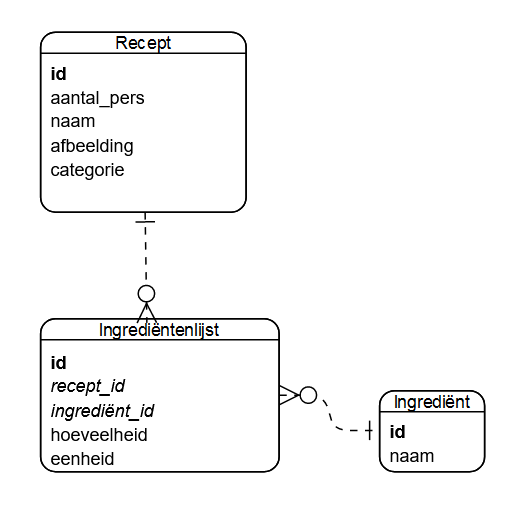
\includegraphics[width=0.7\linewidth]{../ERD}
    \caption[ERD Databank]{ERD voor de databank van recepten}
    \label{fig:erd}
\end{figure}


We nemen 2 willekeurige Belgische websites als proef en zoeken naar de HTML-tags waarin de door ons gezochte inhoud zit. In beide gevallen zijn de recepten zodanig gestructureerd dat de gewenste inhoud snel terug te vinden is a.d.h.v. duidelijke klassen (zoals `recipe-content\_body`) voor de bereidingswijze op een van de sites. Met de Python-bibliotheek `Beautiful Soup` kan de DOM-tree van een website worden overlopen om rauwe data te destilleren. De URL's van de te scrapen pagina's zijn te vinden in de sitemap (indien toegankelijk).  Er dienen nog enkele bewerkingen te gebeuren op de verzamelde data: de categorieën moeten bijgehouden worden bij het recept en de ingrediënten hebben aanpassingen nodige zodanig dat verschillende schrijfwijzen worden toegewezen aan 1 ingrediënt (tomaten en tomaatjes moeten geïdentificeerd worden als tomaat). Dezelfde techniek wordt gebruikt wanneer de gebruiker een ingrediënt invoert.

De gerechten moeten worden onderverdeeld in categorieën. Dit is nodig om later voor een ingrediënt de best passende andere ingrediënten te vinden (deze score wordt berekend binnen een categorie, en een andere categorie geeft andere ingrediënten als best passend). De volgende categorieën zijn van toepassing: vlees, vis, gevogelte, wild, vegetarisch, salade, pasta, ovenschotel. Deze lijst kan worden uitgebreid en ieder recept kan in verschillende categorieën zijn opgenomen. Hoe meer recepten er in zo'n categorie thuishoren, hoe accurater de typicaliteitsscore \autocite{Yokoi2015} later kan worden berekend zonder in te boeten op variatie. Gerechten die niet kunnen worden onderverdeeld in een van deze categorieën (mogelijks ontbreekt er een onderverdeling op de bronwebsite) worden verzameld in een algemene categorie (“hoofdgerecht”). Deze recepten kunnen bij uitbreiding nog gecategoriseerd worden (door bv. te zoeken naar sleutelwoorden zoals `pasta` of `kip`) ter onderhoud van de toepassing.
Een ingrediënt moet worden getransformeerd zodat de gebruikte ingrediënten uniek terug te vinden zijn in onze ingrediëntentabel. Een nuttige techniek die kan worden toegepast is beschreven door \textcite{Chaudhuri2003} en heet “fuzzy matching”.  

Deze techniek vergelijkt een nieuw ingrediënt met de reeds (in enkelvoud) opgeslagen ingrediënten. Er zijn 2 parameters die de performantie beïnvloeden: de grenswaarde en similariteitsfunctie. Deze laatste berekent een score die aangeeft hoe verwant 2 woorden zijn. Wanneer deze score boven een bepaalde grenswaarde valt spreken we van een match. Het nieuwe ingrediënt wordt in dat geval vervangen door de naam van het eerder opgeslagen ingrediënt. Voor twijfelgevallen over de juiste transformatie (“spruit” matcht even goed met “druif” als met “pruim” wanneer edit distance \autocite{Chaudhuri2003} de gebruikte functie is) wordt er gebruik gemaakt van een logbestand om gericht te kunnen debuggen. Het kan interessant zijn om een bepaald interval in te stellen waarin alle twijfelgevallen manueel moeten worden beoordeeld om zo de ideale grenswaarde te vinden. De volgende figuur visualiseert de werkwijze voor een lijst van 5 ingrediënten voor de categorie `hamburger` (deze categorie wordt niet gebruikt in onze toepassing)

Op deze moment hebben we een aantal recepten, voorzien van een titel, foto, ingrediëntenlijst en bereidingswijze. Ze zijn voorzien van één of meerdere categorieën. De ingrediënten die terug te vinden zijn in de receptenlijst zijn getransformeerd naar een uniek ingrediënt uit de ingrediëntentabel waarnaar in het recept wordt verwezen met een vreemde sleutel. Voor de bereidingswijze kan er worden gewerkt met een stappenplan, maar in de scope van dit onderzoek wordt deze als volle tekst gebruikt zoals ze van de site wordt gehaald. Indien de website een bereiding toch onderverdeelt worden alle onderdelen samengevoegd tot 1 veld om compatibel te zijn met de databank.

\subsection{Ingredient matching}%

Voor de volgende stap worden alle recepten onderverdeeld per categorie met elk diens typerende ingrediënten. We willen een score toewijzen aan een verzameling daarvan voor een bepaalde categorie die verhoogt naarmate de combinatie van ingrediënten erbinnen vaak voorkomt. De werkwijze die wordt gehanteerd is beschreven door \textcite{Yokoi2015}.

Ieder recept heeft een overeenstemmende vector die aanduid waaruit het bestaat. Deze heeft een lengte gelijk aan het aantal verschillende ingrediënten in de databank en de aan- of afwezigheid van een bepaald ingrediënt wordt aangeduid met resp. 1 of 0. Al deze vectoren worden samengevoegd tot een matrix met  corresponderende eigenruimte (de numpy-bibliotheek Linear Algebra bevat een methode om deze te berekenen in python). De typicaliteitsscore van een nieuwe ingrediëntvector  \autocite{Yokoi2015} is de L2-norm van diens genormaliseerde projectie op de eigenruimte \autocite{Karabiber}. De waarde ligt tussen 0 en 1 en een hoger getal wijst erop dat de ingrediënten sterk vertegenwoordigd zijn binnen de categorie.\begin{figure}
    \centering
    \includegraphics[width=0.7\linewidth]{"../Voorbeeld opmaken ingrediëntenlijst"}
    \caption[Voorbeeld van het samenstellen van een ingrediëntenlijst]{Voorbeeld van het samenstellen van een ingrediëntenlijst. Merk op dat er in het voorbeeld 5 i.p.v. 4 ingrediënten worden gematcht voor de categorie 'hamburger'' \autocite{Yokoi2015}}
    \label{fig:voorbeeld-opmaken-ingredientenlijst}
\end{figure}

Tot slot implementeren we een manier om de gebruikersvoorkeuren te laten meespelen. Hiervoor meten we hoe vaak een ingrediënt voorkomt in eerder klaargemaakte bereidingen, waarbij diegene die nog niet gebruikt zijn niet in rekening worden gebracht. De typicaliteitsscore wordt verzwaard met het gemiddelde van deze verhoudingen, om de uiteindelijke score te verkrijgen.

Het is deze score die moet worden geoptimaliseerd om een goede match te krijgen. Er moeten verschillende combinaties van 4 ingrediënten worden uitgeprobeerd (waarin hetgeen aangegeven door de gebruiker steeds is ingevuld) totdat een vastgelegde grenswaarde is overschreden. Dit garandeert ons dat niet 1 beste match steeds naar voor komt maar een groep waaruit werd gekozen. De input wordt gebruikt als beginwaarde, de overige 3 elementen van de rij worden willekeurig geïnitialiseerd, om vervolgens één voor één te worden vervangen door een willekeurig ander element uit de ongebruikte verzameling. 

\subsection{Recepten voorstellen}%

In het vorige onderdeel zijn we gestart van 1 ingrediënt dat de gebruiker invoert om een verzameling van 4 stuks te verkrijgen. Omdat deze allemaal in de eerste stap zijn omgevormd naar een geldige referentie kan op basis van daarvan een opzoeking gebeuren in de databank. Het is niet nodig om ook de bereidingsstappen te doorzoeken aangezien de sleutelwoorden waarop we zoeken allemaal te vinden zijn in de ingrediëntenlijst van een recept. In dit stadium zijn er verschillende mogelijke uitkomsten als uitvoer:

\begin{itemize}
    \item Er wordt 1 gerecht geretourneerd
    \item Er wordt een gerecht geretourneerd van iedere categorie waaruit 1 wordt geselecteerd door de gebruiker
    \item Er wordt een gekozen aantal gerechten voorgesteld als weekmenu
\end{itemize}

In het eerste geval hebben we als uitkomst van stap 2 een ingrediëntenlijst per categorie. Doordat de lijst voortkomt uit een groep van matches zijn kan de match met de hoogste score worden gekozen zonder dat dit steeds hetzelfde resultaat geeft. Een alternatieve strategie is dat er geen keuze wordt gemaakt door het systeem, maar dat alle categorieën worden vertegenwoordigd door 1 zoekresultaat waarna de gebruiker één selecteert.
Beide opties geven geen meerwaarde tegenover een woordgebaseerde zoekopdracht, behalve dat de opzoeking kwalitatieve beperkingen respecteert die relevante suggesties voortbrengen. Om die reden wordt er in de toepassing een functionaliteit toegevoegd die de resultaten uitbreidt; Bij een geselecteerd gerecht worden er een gekozen aantal bereidingen toegevoegd om zo een weekmenu tot stand te brengen. Dit menu bestaat uit een gekozen aantal recepten (max. 5) en een chronologische volgorde die stelt welk gerecht op welke dag wordt klaargemaakt. Om ervoor te zorgen dat er voldoende variatie is willen we aan de combinatie van deze gerechten een score toewijzen die aangeeft in hoeverre ze verschillen van elkaar. Een hogere score betekent veel variatie, en dat is wenselijk in een gezond eetpatroon. 
De methode die in het onderzoek wordt gebruikt is een implementatie beschreven door \textcite{Ueda2011}. Naar analogie met de typicaliteitsscore krijgt ieder recept een score die gebruikersvoorkeuren in rekening brengt. Ingrediënten die vaak voorkomen in de lijst van bereidingen die de gebruiker eerder heeft klaargemaakt verhogen de score, terwijl deze die voorkomen in de lijst van ongewenste maaltijden de score verlagen. Ieder voorkomen wordt gekwantificeerd op basis van TF-IDF \autocite{Karabiber2024}. Deze intrinsieke score wordt verminderd met een gewogen score die een maat is voor de (tekstuele) gelijkenis tussen 2 gerechten. Het gewicht neemt af naarmate de gerechten verder van elkaar liggen in de tijd. \textcite{Ueda2011} definieert de volgende formule:

\begin{equation}
    Score(R) = \sum_{k \in R}I_k - \alpha \sum_{d=1}(w_d \cdot sim(R,R_d))
\end{equation}

Door de scores op te tellen bekomen we een maat voor de variatie die nog steeds rekening houdt met gebruikersvoorkeuren. Deze score kan worden geoptimaliseerd op 2 manieren: ofwel wordt het beste volgende gerecht iteratief aan het menu toegevoegd tot het gewenste aantal is bereikt, ofwel worden alle mogelijke combinaties uit de eerder gevonden bereidingen gecombineerd en blijft de combinatie met de hoogste score behouden. We beperken ons tot het opstellen van een weekmenu met max. 5 maaltijden met 2 voorgestelde gerechten per categorie om de bewerkingstijd te beperken.

\section{Verwachte resultaten}%
\label{sec:verwachte-resultaten}

% TODO: (fase 6 - afwerking)

Het verwachte resultaat is dat het toepassen van de beschreven technieken de relevantie van voorgestelde gerechten verhoogd. Het meten van relevantie is echter subjectief (de criteria waarop een waardering zich baseert zijn uiteenlopend en kunnen verschillen naargelang het moment), waardoor we dit niet kunnen gebruiken als leidraad. Ook wordt er aangenomen dat door gericht te zoeken de resultaten verbeteren, wat niet bewezen is. We moeten vermijden dat de situatie zich voordoet waarbij onze methode werkt, maar dit tegengesproken wordt door tegenvallende waarderingen. 

Het nut van de toepassing kan worden aanzien in termen van conversie. Doordat historische voorkeuren in kaart worden gebracht horen de resultaten doorheen de tijd nauwer samen te vallen met de wensen van de gebruiker. We verwachten dat het herhaaldelijk gebruik zich vertaalt in een grotere kans dat voorgestelde recepten worden klaargemaakt, en een kleinere kans dat een recept wordt afgewezen. We stellen arbitrair dat bij het eerste gebruik de conversie ongeveer 60\% hoort te zijn om te spreken van een nuttig voorstel, en dat dit door herhaaldelijk gebruik hoort te stijgen. Als dit het geval is kunnen we stellen dat de toepassing een meerwaarde biedt. Omdat het niet duidelijk is of de resultaten normaal zijn verdeeld dient de t-test te worden gebruikt om een beeld te geven van hoe significant een trend is.

\section{Discussie, verwachte conclusie}%
\label{sec:discussie-conclusie}

Het doel van de toepassing is het faciliteren van het proces om geschikte maaltijden voor te stellen, gebruik makende van gerichte opzoekingen in een databank op maat van de gebruiker. Eerder gebruikte ingrediënten worden in rekening gebracht, er is een manier om voor een aantal gecombineerde gerechten een grote variëteit te bewaken, in verschillende categorieën worden ingrediënten met elkaar gecombineerd gebaseerd op hoe frequent ze samen voorkomen én de zoekresultaten maken gebruik van gebruikersinvoer. In het proces zijn er een aantal keuzes gemaakt die van grote invloed zijn op het resultaat, en het is van groot belang om na te gaan welke optimalisaties er mogelijk zijn door deze parameters te laten variëren, wat zou kunnen worden aangegrepen als toekomstig werk. Enkele voorbeelden:

\begin{itemize}
    \item de bronwebsites bepalen de zoekresultaten en dus mogelijks de relevantie voor een gebruiker
    \item de grenswaarde van typicaliteit \autocite{Yokoi2015} waarboven een verzameling ingrediënten geldig is. Hoe lager deze waarde, hoe minder nauw de ingrediënten verbonden zijn, maar hoe meer mogelijke gerechten er kunnen worden voorgesteld
    \item de parameter $\alpha$ bij het combineren van recepten bepaalt de mate waarin een gelijkaardig gerecht als negatief wordt beschouwd
    \item het aantal recepten per categorie waaruit wordt gekozen
    \item ...
\end{itemize}

Om ingrediënten en recepten met elkaar te vergelijken is er steeds gebruik gemaakt van tekstuele informatie. Het aantal voorkomens van woorden wordt gebruikt, zonder rekening te houden met intrinsieke eigenschappen die van belang kunnen zijn. Zo wordt de smaak nooit gekwantificeerd, terwijl er een hele wetenschap schuil gaat achter food pairing \autocite{Ahn2011}. Het implementeren van dergelijke manieren om ingrediënten te matchen zou de relevantie nog kunnen verbeteren. 


%------------------------------------------------------------------------------
% Referentielijst
%------------------------------------------------------------------------------
% TODO: (fase 4) de gerefereerde werken moeten in BibTeX-bestand
% bibliografie.bib voorkomen. Gebruik JabRef om je bibliografie bij te
% houden.

\printbibliography[heading=bibintoc, title={References}] 

\end{document}